%
%	Begrifflichkeiten
%

\pagebreak
\section{Targeting}

\onehalfspacing

\subsection{Targeted Advertising}

\subsubsection{Rationale}

To be written.

\subsubsection{Tracking}

To be written.

\subsubsection{Cookies}

To be written.

\subsection{Data Types}

\subsubsection{First-Party Data}

To be written.

\subsubsection{Second-Party Data}

To be written.

\subsubsection{Third-Party Data}

To be written.

\subsection{Toolstacks}

\subsubsection{Google Analytics}

To be written.

\begin{figure}[H]
\centering
\caption {Plausible}
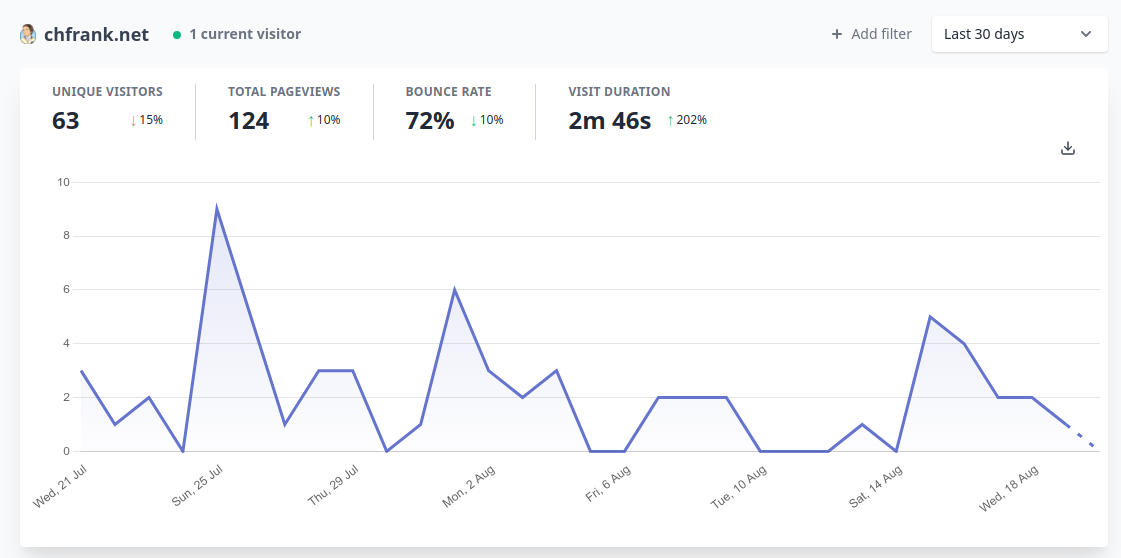
\includegraphics[width=\linewidth]{images/plausible.png}
\label{fig:plausible}
\end{figure}

\subsubsection{Google Ads and AdWords}

To be written.

\subsubsection{Amazon Advertising}

To be written.

\subsubsection{Facebook Advertising}

To be written.

\subsubsection{Yandex Metrica}

To be written.

\subsection{Moving past cookies}

\subsubsection{Google FLoC}

To be written.

\subsubsection{UID2}

To be written.

\subsubsection{Microsoft Parakeet}

To be written.

\subsubsection{Apple Identifier for Advertisers (IDFA)}

To be written.

\subsubsection{Android Advertising ID (AAID) / Google Advertising ID (GAID)}

To be written.

\subsubsection{Content-based targeting}

To be written.

\subsection{Legal Framework}

\subsubsection{GDPR (General Data Protection Regulation) / UK-GDPR}

To be written.

\subsubsection{DS-GVO (Datenschutz-Grundverordnung)}

To be written.

\subsubsection{EU e-Privacy Proposal}

To be written.

\subsubsection{Telekommunikations-Telemedien-Datenschutz-Gesetz (Entwurf)}

To be written.

\subsubsection{Other Legal Frameworks}

\begin{itemize}
 \item CCPA (California Consumer Privacy Act)
 \item LGPD (Lei Geral de Proteção de Dados Pessoais)
 \item POPIA (Protection of Personal Information Act)
 \item DSA (Digital Services Act)
 \item DMA (Digital Markets Act)
\end{itemize}


